% Author @ Jeremy Perez, UNDER-REVIEW, Reviewer @ Claudia Porto

A* is a much more sophisticated graph traversing algorithm capable of finding the shortest path between two nodes. Before formally defining it, there exists some additional concepts which prove to be important when understanding it's adoption in this study.

\subsubsection{Problem Modeling}

Any problem can be modeled by formally defining the following:
\begin{enumerate}
    \item \textbf{Initial States}: What initial state can an algorithm begin with?
    \item \textbf{Possible actions}: What \textbf{actions} can be taken given the current state?
    \item \textbf{Successor Function} What state is an algorithm in after it performs an action?
    \item \textbf{Goal Test}: Is the current state the goal state of the problem?
\end{enumerate}

\noindent This formulation is commonly defined using the notion of an \textit{agent} but for the sake of conciseness, we have restricted its definition to mean just algorithm, given the fact that we'll be formulating problems for algorithms to solve.



\subsubsection{State Spaces}
A \textbf{state space} is a structure that represents all possible configurations of a problem. Formally it is defined using a tuple $(N,E,S,G)$ where:

\begin{itemize}
    \item $N$ is the set of states.
    \item $E$ is the set of directed edges connecting states.
    \item $S \subseteq N$ is a nonempty set that contains the starting states.
    \item $G \subseteq N$ is a nonempty set that contains a goal state.
\end{itemize}

\noindent
These structures can be quite useful for testing decision-making strategies on a problem.

Let's work through a concrete example. Suppose you are getting ready for work and you notice that you are barefoot. You task yourself with putting on a single shoe first. If we were to observe the state space of putting on a shoe, we get that:
\begin{itemize}
    \item $N =$ \{bareFoot, sockOnFoot, shoeOn\})
    \item $E =$ \{(bareFoot, sockOnFoot), (sockOnFoot,bareFoot), (sockOnFoot,shoeOn), (shoeOn,sockOnFoot)\})
    \item $S =$ \{bareFoot\}
    \item $G =$ \{shoeOn\}
\end{itemize}

\begin{center}
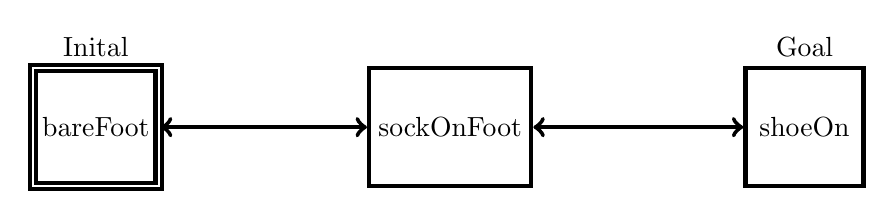
\begin{tikzpicture}[scale=1.5]
    % Draw nodes for V1
    \node[ultra thick ,double, minimum size=1.5cm, draw,label=above:{Inital}] (1) at (0, 0) {bareFoot};
    \node[ultra thick,minimum size=1.5cm, draw] (2) at (3, 0) {sockOnFoot};
    \node[ultra thick,minimum size=1.5cm, draw,label=above:{Goal}] (3) at (6, 0) {shoeOn};

    % Draw edges
    \draw[ultra thick, <->] (1) -- (2) ;
    \draw[ultra thick, <->] (2) -- (3);
\end{tikzpicture}
\end{center}
\noindent
Notice that in this example, you are not able to directly go from being bareFoot to a state of being with a shoeOn. 
It requires going to a state of sockOnFoot first. By design, this 
model embeds every action possible
at any given time. It essentially is capable of making any decision-based problem into a graph problem.

\subsubsection{Problem Modeling of Maximum Matching}
Applying these concepts to the Maximum Matching problem, let us begin by observing what some formulations of this problem look like. Usually, the largest difference between Maximum Matching formulations is the representation of states. Because of the existence of reductive solutions, formulations can vary greatly. Here are some simple ones:
\begin{itemize}
    \item \textbf{Subset Formulation}: Assume you begin with the graph $G=(V,E)$ where $V$ denotes the set of vertices and $E$ denotes the set of edges.
Suppose your initial state is the entire edge-set $E$.
Let the possible actions at any state be removing any of the edges in the current edge set of the state. Let the successor function remove the edge out of the set. 
The goal test is whether or not the current state's edge set is a maximum matching of $G$. 
\item \textbf{Superset Formulation}: Assume you begin with the graph $G=(V,E)$ where $V$ denotes the set of vertices and $E$ denotes the set of edges, suppose your initial state's edge-set is the empty set $\emptyset$.
Let the possible actions at any state add an edge from $E$ which is not currently present in the edge set. Let the successor function add the chosen edge to the edge set. 
The goal test is whether or not the current state's edge set is a maximum matching of $G$. 
\end{itemize}


\noindent Using Figure~\ref{fig:subsetStates} to visualize the structure of a Max Matching State Space, we uncover that there exists some underlying mathematical relationships to these types of structures. The states in this space directly correspond to the elements of the \textbf{Power Set} of $E$, denoted $\mathcal{P}(E)$, which is the set of all possible subsets of a set. This set has a cardinality of $2^{|E|}$.

Notice that the Superset formulation can be articulated by flipping the goal and initial states and flipping the direction of every transition in the state space of the Subset formulation. These formulation directly relates to power sets being \textit{Boolean algebras} under normal set operations and boolean algebras having a \textit{dual}. This explains why the state space forms a lattice-like structure. Useful properties of these mathematical structures may prove to be helpful at developing refined renditions of this problem.

\begin{figure}
\centering
\begin{tikzpicture}[
node distance = 15mm and 20mm,
  start chain = going right,
     N/.style = {inner sep=1pt, on chain,minimum size=1cm, draw},
                    ]
\node (n21) [N] {...};
\node (n22) [N] {...};
\node (n23) [N] {...};
\node (n24) [N] {...};
\node (n25) [N] {...};
%
\node (n11) [N, label=left:{Removed Edges: $m-1$}, below=of n21]           {$\{e_m\}$};
\node (n12) [N, below=of n22] {$\{e_{m-1}\}$};
\node (n13) [N, below=of n23]{$...$};
\node (n14) [N, below=of n24] {$\{2\}$};
\node (n15) [N, below=of n25] {$\{1\}$};
%
\draw [<-](n11) -- (n21);
\draw [<-](n11) -- (n22);
\draw [<-](n11) -- (n23);
\draw [<-](n11) -- (n24);
\draw [<-](n11) -- (n24);
\draw [<-](n11) -- (n25);
\draw [<-](n12) -- (n21);
\draw [<-](n12) -- (n22);
\draw [<-](n12) -- (n23);
\draw [<-](n12) -- (n24);
\draw [<-](n12) -- (n24);
\draw [<-](n12) -- (n25);
\draw [<-](n13) -- (n21);
\draw [<-](n13) -- (n22);
\draw [<-](n13) -- (n23);
\draw [<-](n13) -- (n24);
\draw [<-](n13) -- (n24);
\draw [<-](n13) -- (n25);
\draw [<-](n14) -- (n21);
\draw [<-](n14) -- (n22);
\draw [<-](n14) -- (n23);
\draw [<-](n14) -- (n24);
\draw [<-](n14) -- (n24);
\draw [<-](n14) -- (n25);
\draw [<-](n15) -- (n21);
\draw [<-](n15) -- (n22);
\draw [<-](n15) -- (n23);
\draw [<-](n15) -- (n24);
\draw [<-](n15) -- (n24);
\draw [<-](n15) -- (n25);
%
\node (n31) [N, label=left:{Removed Edges: 1}, above=of $(n21.south)!0.5!(n22.south)$]  {$\{e_2,e_3,...,e_m\}$};
\node (n32) [N, above=of n23]  {...};
\node (n33) [N, above=of $(n24.south)!0.5!(n25.south)$]  {$\{e_1,e_3,...,e_{m-1}\}$};
%
\draw [->](n31) -- (n21)    ;
\draw [->](n31) -- (n22)  ;
\draw [->](n31) -- (n23) ;
\draw [->](n31) -- (n24) ;
\draw [->](n31) -- (n25);
\draw [->](n32) -- (n21)    ;
\draw [->](n32) -- (n22)  ;
\draw [->](n32) -- (n23) ;
\draw [->](n32) -- (n24) ;
\draw [->](n32) -- (n25);
\draw [->](n33) -- (n21)    ;
\draw [->](n33) -- (n22)  ;
\draw [->](n33) -- (n23) ;
\draw [->](n33) -- (n24) ;
\draw [->](n33) -- (n25);
;
%
\node (n41) [N, double, label=above:{Inital}, above=of $(n32.north)$] {$\{e_1,e_2,...,e_m\}$};
%
\draw [->](n41) -- (n31);  
\draw [->](n41) -- (n32);
\draw [->](n41) -- (n33);
%
\node (n51) [N, below=of n13] {$\emptyset$};
%
\draw [<-](n51) -- (n11);
\draw [<-](n51) -- (n12);
\draw [<-](n51) -- (n13);
\draw [<-](n51) -- (n14);
\draw [<-](n51) -- (n15);
\end{tikzpicture}
\caption{This is a visualization of the state space of a Maximum Matching problem using the Subset Formulation.}
\label{fig:subsetStates}

\end{figure}






\subsubsection{Optimizing State Spaces}
As foreshadowed, it is possible to truncate state spaces for the sake of optimizing traversal strategies. For instance, using the fact that the maximum matching is always $n$ (the number of vertices) or less means a new problem formulation of the problem can be made by removing all states where the edge-set is bigger than $n$. The resulting state space would then have initial states starting with edge sets with $n$ elements. Applying this to the subset formulation of maximum matching, we would get a smaller subspace that looks like Figure~\ref{fig:truncatedStates}

\begin{figure}
    \centering
    
\begin{tikzpicture}[
node distance = 10mm and 5mm,
  start chain = going right,
     N/.style = {inner sep=1pt, on chain,minimum size=1cm, draw},
                    ]
\node (n21) [N] {...};
\node (n22) [N] {...};
\node (n23) [N] {...};
\node (n24) [N] {...};
\node (n25) [N] {...};
%
\node (n11) [N, label=left:{Removed Edges: $m-1$}, below=of n21]           {$\{e_m\}$};
\node (n12) [N, below=of n22] {$\{e_{m-1}\}$};
\node (n13) [N, below=of n23]{$...$};
\node (n14) [N, below=of n24] {$\{2\}$};
\node (n15) [N, below=of n25] {$\{1\}$};
%
\draw [<-](n11) -- (n21);
\draw [<-](n11) -- (n22);
\draw [<-](n11) -- (n23);
\draw [<-](n11) -- (n24);
\draw [<-](n11) -- (n24);
\draw [<-](n11) -- (n25);
\draw [<-](n12) -- (n21);
\draw [<-](n12) -- (n22);
\draw [<-](n12) -- (n23);
\draw [<-](n12) -- (n24);
\draw [<-](n12) -- (n24);
\draw [<-](n12) -- (n25);
\draw [<-](n13) -- (n21);
\draw [<-](n13) -- (n22);
\draw [<-](n13) -- (n23);
\draw [<-](n13) -- (n24);
\draw [<-](n13) -- (n24);
\draw [<-](n13) -- (n25);
\draw [<-](n14) -- (n21);
\draw [<-](n14) -- (n22);
\draw [<-](n14) -- (n23);
\draw [<-](n14) -- (n24);
\draw [<-](n14) -- (n24);
\draw [<-](n14) -- (n25);
\draw [<-](n15) -- (n21);
\draw [<-](n15) -- (n22);
\draw [<-](n15) -- (n23);
\draw [<-](n15) -- (n24);
\draw [<-](n15) -- (n24);
\draw [<-](n15) -- (n25);
%
\node (n31) [N, label=above:{Initial},label=left:{Removed Edges: $(m-n)$}, above=of n21]  {$\{e_1,e_2,...,e_n\}$};
\node (n32) [N, label=above:{Initial},above=of $(n23.north)$]  {...};
\node (n33) [N, label=above:{Initial},label=right:{\# of States in Level $= \binom{m}{n}$ },above=of n25]  {$\{e_{m-n},e_{m-n+1},...,e_{m}\}$};
%
\draw [->](n31) -- (n21)    ;
\draw [->](n31) -- (n22)  ;
\draw [->](n31) -- (n23) ;
\draw [->](n31) -- (n24) ;
\draw [->](n31) -- (n25);
\draw [->](n32) -- (n21)    ;
\draw [->](n32) -- (n22)  ;
\draw [->](n32) -- (n23) ;
\draw [->](n32) -- (n24) ;
\draw [->](n32) -- (n25);
\draw [->](n33) -- (n21)    ;
\draw [->](n33) -- (n22)  ;
\draw [->](n33) -- (n23) ;
\draw [->](n33) -- (n24) ;
\draw [->](n33) -- (n25);
;

%
\node (n51) [N, below=of n13] {$\emptyset$};
%
\draw [<-](n51) -- (n11);
\draw [<-](n51) -- (n12);
\draw [<-](n51) -- (n13);
\draw [<-](n51) -- (n14);
\draw [<-](n51) -- (n15);
\end{tikzpicture}


    \caption{Truncated version of Figure~\ref{fig:subsetStates} where the first $m-n-1$ levels were removed and each proceeding leaf state from it's bottom most level has become initial states. }
    \label{fig:truncatedStates}
\end{figure}    


\subsubsection{Traversal Strategies to Find Solution States}

Strategies for traversing state spaces to find solutions (analogous to finding goal states) are broken into two major classifications: 
\begin{itemize}
    \item \textbf{Uninformed search} strategies refer to algorithms that traverse state spaces without any more information about states beyond what is specified in the problem. All that is known to these algorithms is whether or not a state is a goal state.  Examples of this include deploying Breadth First Search, Iterative deepening search, or Bidirectional Search on the state space to find solutions.
    \item \textbf{Informed search}, also known as \textbf{Heuristic search}, refers to algorithms that use additional information, beyond a problem formulation, to decide how to traverse state spaces. 
\end{itemize}

\noindent In the example of using breadth-first search, this is exactly what the un-pruned brute force algorithm is. Its runtime has a known worst-case running time of $O(2^m)$ and corresponds to the algorithm traversing through every state mentioned in the Subset Formulation of the problem. 


\subsubsection{Best-First Search and A*}

\textbf{Best-First} search is the most common form of informed search.
It utilizes an \textbf{evaluation function} to calculate a state's
\textit{costliness} and expands nodes that are the cheapest. Please refer to Figure~\ref{fig:BestFirst}
 to see a quick example.

The evaluation function estimates cost using various factors and is often a composition of functions.


One function commonly found inside the evaluation function is the heuristic component/function. A \textbf{heuristic function} given a state, calculates an estimated cheapest cost to the remaining distance to a goal state. A good way to think about this is that it's a value associated with the remaining "distance" to an answer. 


\begin{figure}
    \centering
    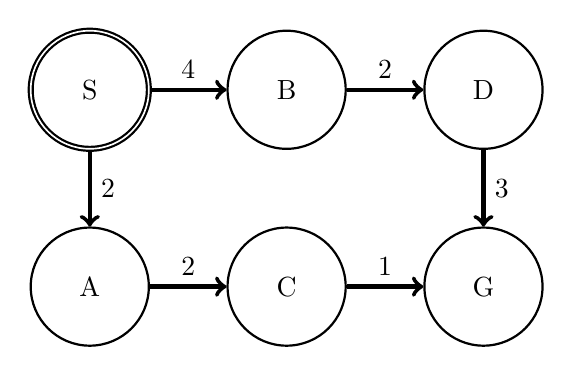
\begin{tikzpicture}[node distance=2.5cm, auto, scale=0.5]
    \node[ double, thick,circle, minimum size=1.5cm, draw] (S) at (0,0) {S};
    \node[ thick,circle, minimum size=1.5cm, draw] (A) [below of=S ] {A};
    \node[ thick,circle, minimum size=1.5cm, draw] (B) [ right of=S] {B };
    \node[ thick,circle, minimum size=1.5cm, draw] (C) [right of=A] {C };
    \node[ thick,circle, minimum size=1.5cm, draw] (D) [right of=B] {D};
    \node[ thick,circle, minimum size=1.5cm, draw] (G) [right of=C] {G};
    
    % Draw the edges
    \path[ultra thick, ->] 
  (S) edge node {2} 
  (A) edge node {4} (B)
  (A) edge node {2} (C)
  (B) edge node {2} (D)
  (C) edge node {1} (G)
  (D) edge node {3} (G);
    
\end{tikzpicture}
    \caption{Let's say we want to find some shortest path from a initial state $S$ to a goal state $G$ using a Best First Search algorithm. In an automaton style of execution, the cheapest action is to go to state $A$. Wholistically, the next cheapest action is to go to state $C$ and again the cheapest action from there is to go to $G$. The order of expansion would be $S,A,C,G$}
    \label{fig:BestFirst}
\end{figure}



\textbf{A* }is a type of Best-First Search Algorithm that traverses through a graph minimizing the total estimated cost. Its evaluation function is the combination of the cost to reach a node and the cost from the node to the goal. Since it's a best-first search algorithm, it's expanding states based upon the cheapest estimated cost of a path going through a state.


\subsubsection*{Optimal Heuristics}
Not all heuristics are equal and finding one which will give a good estimation of the remaining short distance to a goal state consistently can be challenging. An \textbf{admissible heuristic} is one that \textit{never overestimates} the cost to reach a goal state. Having a heuristic which fulfills this property ensures that $A^*$ will reach a correct solution consistently.

\subsubsection*{Future Works}
\subsubsection*{Isomorphism Optimization of State Space}

An additional way we conjectured to truncate state spaces is with the usage of \textbf{Graph isomorphisms}. Graph Isomorphisms are useful functions that when built show that some properties of one graph are present in another. The whole reasoning behind this optimization is that two graphs that are \textit{isomorphic} to each other will have the same Maximum Matching. To put it simply, two graphs that look like each other should have the same matching. 
With the usage of a memoization table, and keeping track of isomorphisms for a graph, the number of states within each level of a state space will be reduced.


\begin{figure}[ht]

\begin{center}
    
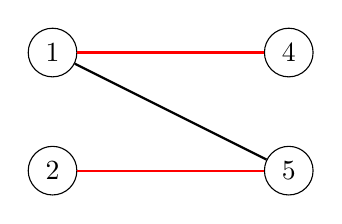
\begin{tikzpicture}[scale=0.75]
    % Draw nodes for set U
    \node[circle, draw] (u1) at (0, 2) {1};
    \node[circle, draw] (u2) at (0, 0) {2};
    % Draw nodes for set V
    \node[circle, draw] (v1) at (4, 2) {4};
    \node[circle, draw] (v2) at (4, 0) {5};

    % Draw all edges (undirected)
    \draw[thick,red] (u1) -- (v1); % Edge between 1 and 4
    \draw[thick] (u1) -- (v2); % Edge between 1 and 5
    \draw[thick,red] (u2) -- (v2); % Edge between 2 and 4

\end{tikzpicture}
\hspace{3cm}
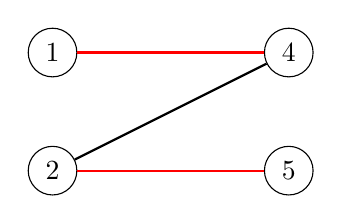
\begin{tikzpicture}[scale=0.75]
    % Draw nodes for set U
    \node[circle, draw] (u1) at (0, 2) {1};
    \node[circle, draw] (u2) at (0, 0) {2};
    % Draw nodes for set V
    \node[circle, draw] (v1) at (4, 2) {4};
    \node[circle, draw] (v2) at (4, 0) {5};

    % Draw all edges (undirected)
    \draw[thick,red] (u2) -- (v2); % Edge between 1 and 4
    \draw[thick] (u2) -- (v1); % Edge between 1 and 5
    \draw[thick,red] (u1) -- (v1); % Edge between 2 and 4

\end{tikzpicture}
\end{center}

 \caption{All though these are technically two different graphs and likewise will be different states, an isomorphism exists between these two graphs, and because of this they will have the same matching}

\end{figure}

\noindent This likely wouldn't lead to a practical computational speed-up but would likely prove to be an informative study that showcases the underlying structures and connections between solutions and the shapes of graphs that will lead to a solution.

